\documentclass[10pt,a4paper]{article}
\usepackage[margin=18mm]{geometry}
\usepackage[T1]{fontenc}
\usepackage{lmodern,microtype}
\usepackage{amsmath,amssymb}
\usepackage{graphicx,booktabs,tabularx,array,longtable,float,caption}
\usepackage[table]{xcolor}
\usepackage{tikz}
\usetikzlibrary{arrows.meta,positioning,calc,shapes.geometric}
\usepackage{pgfplots}
\pgfplotsset{compat=1.18}
\usepackage{csquotes}
\usepackage[colorlinks=true,linkcolor=blue!55!black,citecolor=blue!55!black,urlcolor=blue!55!black]{hyperref}
\usepackage[backend=biber,style=ieee,sorting=none,doi=true,url=false]{biblatex}
\addbibresource{references.bib}
\definecolor{mpblue}{RGB}{28,63,87}
\definecolor{mpteal}{RGB}{18,118,132}
\definecolor{mpgold}{RGB}{183,110,47}
\definecolor{mplight}{RGB}{239,247,249}
\definecolor{mpcream}{RGB}{254,246,235}
\setlength{\parindent}{0pt}
\setlength{\parskip}{4pt}
\renewcommand{\arraystretch}{1.20}
\emergencystretch=3em
\captionsetup{font=small}
\newcommand{\MP}{microplastic}
\newcommand{\tracka}{\textbf{Track A (live boat sensing)}}
\newcommand{\trackb}{\textbf{Track B (geotagged collection + shoreline processing)}}
\title{\bfseries Microplastic Concentration Mapping in Freshwater\\[4pt]
\large Two Practical Measurement Tracks: Live Boat Monitoring and Portable Shoreline Post-processing}
\author{Year 3 Group Project -- Working background and concept-selection review}
\date{October 2026}
\begin{document}
\maketitle
\begin{abstract}
This revised background review combines the previously screened freshwater literature with the stakeholder's requirement to produce a portable, automated, two-dimensional map of microplastic (MP) concentration. Two workflows are evaluated: (A) real-time measurements from a boat and (B) geotagged water collection with rapid, self-contained processing at the shoreline. \textbf{Routine access to FTIR, Raman, or a chemistry laboratory is not assumed.} Camera-assisted particle counting, flow imaging, electrical impedance, fluorescence, polarisation, and water-quality proxies are compared by operating principle, deployment effort, specificity and evidence. A staged decision plan is proposed to distinguish \emph{suspected particle concentration} from a defensible \emph{microplastic concentration} estimate. Paper counts in this review are preliminary keyword-screening outcomes rather than demonstrated method performance.
\end{abstract}

\section{Stakeholder requirements and scope}
The stakeholder brief calls for a system that estimates microplastic concentration over a lake or river surface, produces a \emph{two-dimensional spatial concentration map}, surveys relatively large areas quickly, is practical to deploy and can be validated against appropriate reference measurements. The briefing explicitly allows direct measurement or image-based methods and a boat or aerial platform. It notes that conventional collection, filtration and microscope counting are slow and have limited spatial coverage. Here we take the boat as the vehicle and reformulate measurement into two feasible deployment tracks. \textbf{A continuous coloured image of water appearance is not, by itself, a validated map of microplastic concentration.} Similarly, GPS only places estimates on a map; it does not establish that they represent plastic particles \cite{Chen2021,Chen2023,Blevins2021}.

The current engineering constraint is that \textbf{routine specialist laboratory access is impractical}. This makes a compact, cleanable, low-maintenance measurement path and a robust portable cross-check especially important. Low-cost field processing can support preliminary concentration estimates, while polymer-specific identification would still need occasional external testing if definitive MP attribution is required.

\subsection{What is meant by concentration?}
For counted particles, the target quantity is $C=N_{\mathrm{MP}}/V_{\mathrm{water}}$ in particles/L, stated for a defined detectable particle-size range and sampling depth. A count of \emph{suspected} MPs inferred from images should be reported as such until specificity has been demonstrated. For model-derived estimates, uncertainty and calibration domain must be reported. Polymer mass concentrations from thermal analysis are a different measurand and cannot simply be substituted for particles/L \cite{Blevins2021,Sefiloglu2024}.

\section{Literature selection and four background themes}
From the prior Web of Science--Scopus search, 18,942 records were identified. After removing 7,318 duplicates and 727 document-type exclusions, 10,897 remained for title/abstract screening; 10,833 were preliminary include candidates and 64 needed manual review. The four theme tags overlap: causes (6,430), water effects (7,575), laboratory/measurement methods (6,654) and data trends/mapping (5,320). These labels do not represent completed full-text eligibility screening.

\begin{figure}[H]\centering
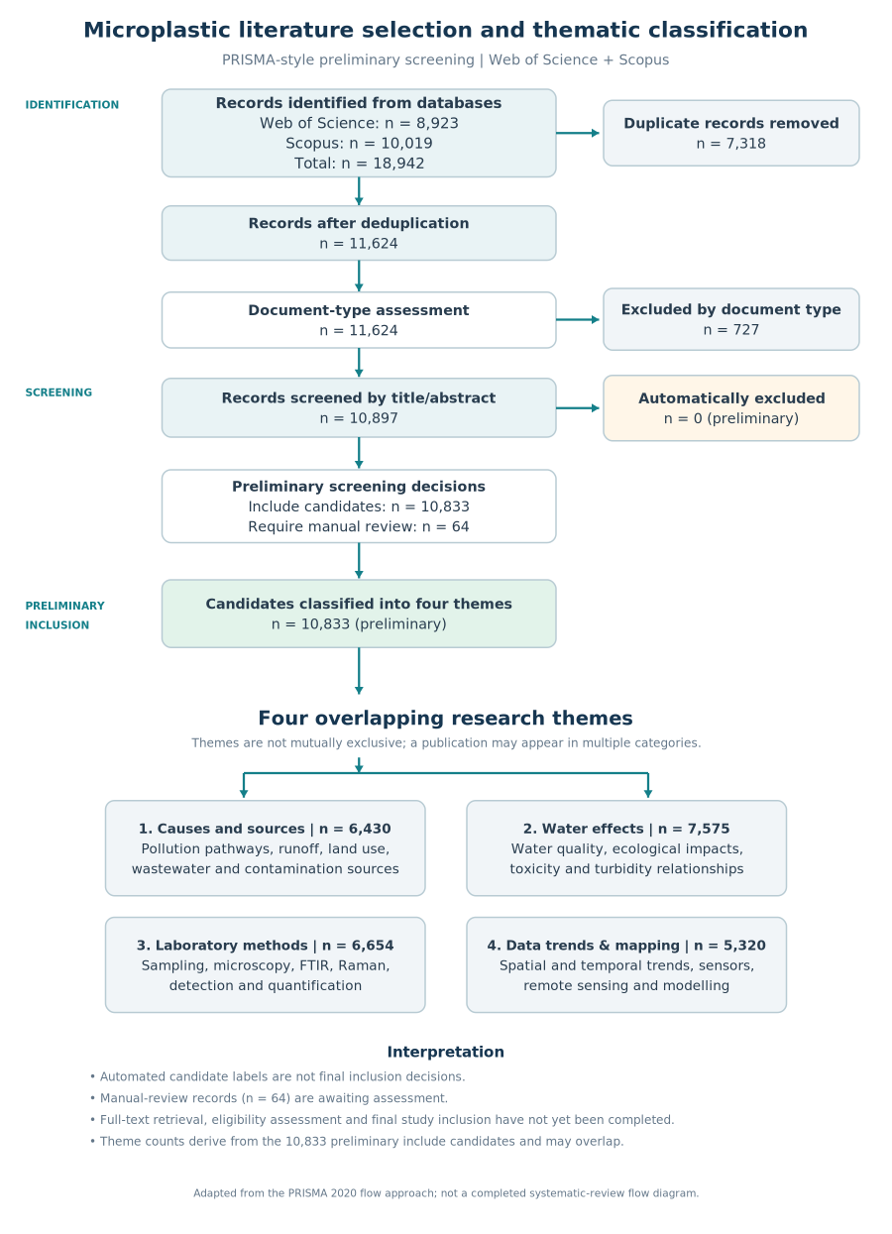
\includegraphics[height=0.55\textheight,keepaspectratio]{Figures/prisma.png}
\caption{Original preliminary screening and four overlapping classifications. Counts are not independent study totals.}\label{fig:prisma}
\end{figure}

\subsection{Sources and causes of riverborne microplastics}
Land use, wastewater, roads, runoff and local discharge influence the spatial distribution of MPs. Tropical river studies illustrate variation between sites and sampling periods rather than one uniform concentration across a catchment \cite{Chen2021,Chen2022,MPWE00007,MPWE00013}. For either track, each measurement must retain sampling location, date, depth and nearby environmental context.

\subsection{Effects and physical/chemical water properties}
Relevant literature covers ecological effects and associations with turbidity, conductivity, suspended solids and nutrients. These properties may influence sensor signals but are \emph{not uniquely attributable to MPs}. For instance, nitrogen/conductivity relationships in surface-water research do not demonstrate a universal electrical MP concentration sensor \cite{MPWE00002,MPWE02100}. Therefore sediment, algae, bubbles, dissolved salts and changing illumination must be tested explicitly as interferents.

\subsection{Measurement and reference methods}
Collection, filtration, microscope imaging, FTIR and Raman feature prominently in the initial screening. Image-based counting can quantify visible particles after appropriate segmentation, whereas spectroscopy can support polymer identity but requires equipment beyond the present project constraint \cite{Ermolin2024,Lee2022,UrbanCNN2024,MPWE00012}. Portable microscope imaging is therefore a feasible preliminary \emph{field-reference} for particle counts, but not a definitive chemical reference for all MPs.

\subsection{Data trends and spatial prediction}
Rivers change with rainfall, flow and location, so isolated point measurements must be mapped with times and uncertainty. Remote imagery and GIS have been explored, but translating visible surface patterns or turbidity into MP particles/L requires paired calibration and external testing \cite{Chen2021,MPWE04211,MPWE02100}. \emph{Track B can create a post-survey heat map from discrete geotagged samples; a heat map does not require that concentrations were measured while the boat was moving.}

\section{Two-track system architecture}
\subsection{Two processes, one map specification}
Figure~\ref{fig:tracks} presents two end-to-end workflows. The diagram is intentionally technology-agnostic: its purpose is to define the operational stages and thereby the criteria used to filter candidate sensing methodologies. The boat and GPS path are shared, but the sensing stage and the downstream handling occur in different places. Track A is more automated and ambitious; Track B is a practical alternative when continuous in-water particle detection is unreliable, too expensive or difficult to maintain.

\begin{figure}[H]\centering
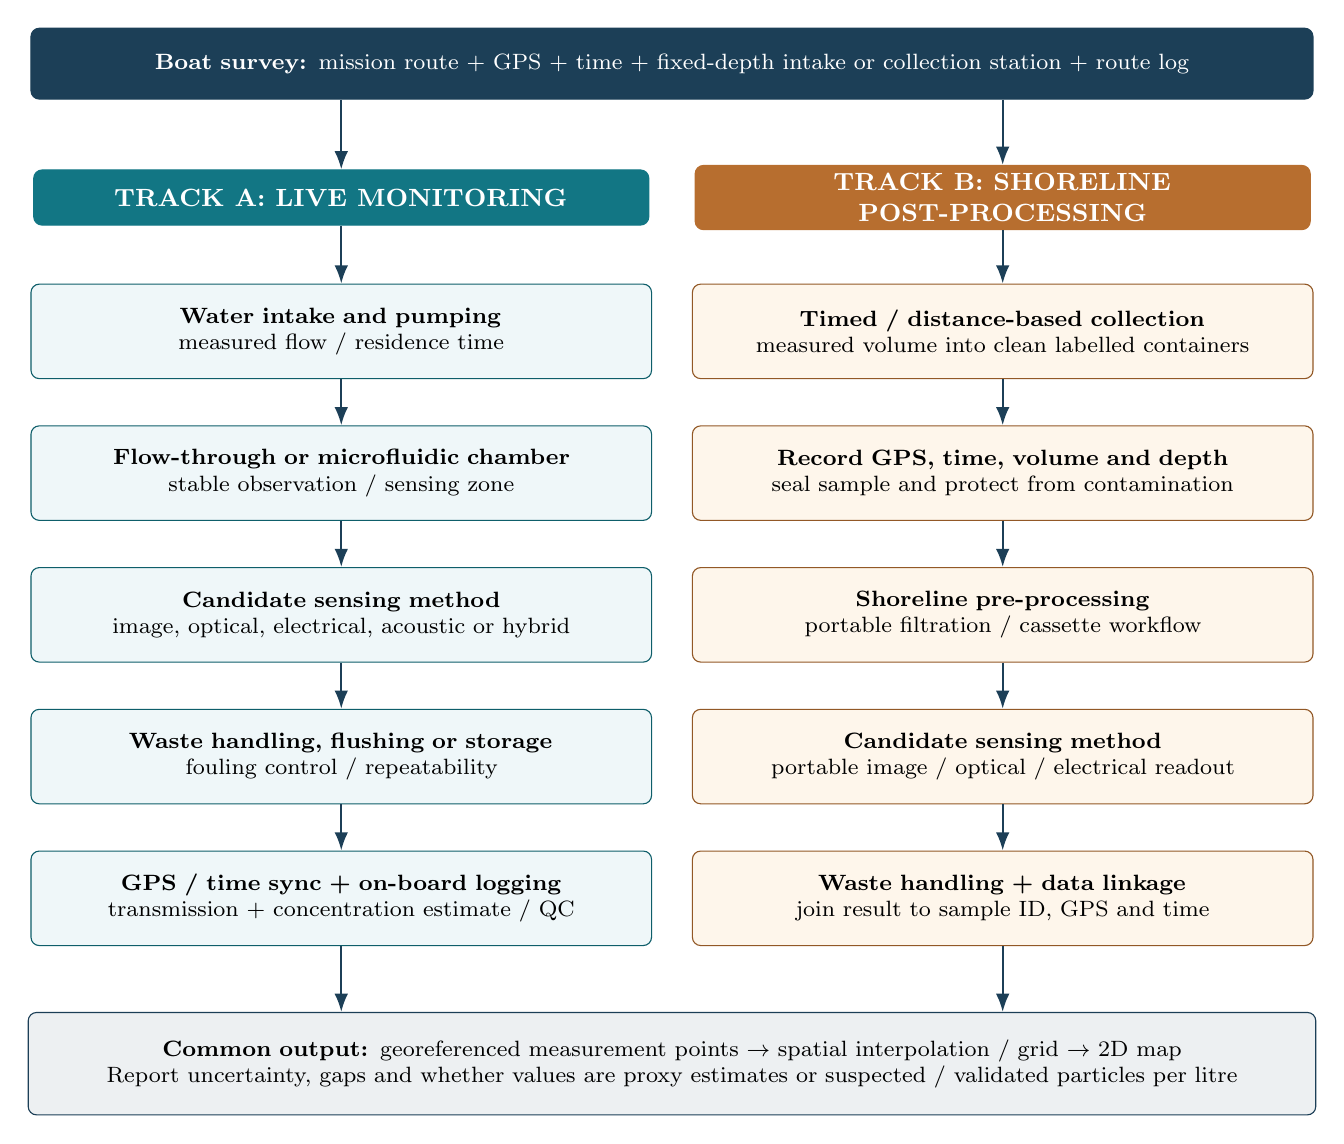
\begin{tikzpicture}[>=Latex, font=\footnotesize,
 % ---- styles ----
 startbox/.style={draw=mpblue,fill=mpblue,text=white,rounded corners=3pt,
   align=center,text width=16cm,minimum height=9mm,inner sep=4pt},
 hdrA/.style={draw=mpteal,fill=mpteal,text=white,rounded corners=3pt,
   align=center,text width=7.6cm,minimum height=7mm,font=\bfseries\small,inner sep=3pt},
 hdrB/.style={draw=mpgold,fill=mpgold,text=white,rounded corners=3pt,
   align=center,text width=7.6cm,minimum height=7mm,font=\bfseries\small,inner sep=3pt},
 stepA/.style={draw=mpteal!80!black,fill=mplight,rounded corners=3pt,
   align=center,text width=7.6cm,minimum height=12mm,inner sep=4pt},
 stepB/.style={draw=mpgold!80!black,fill=mpcream,rounded corners=3pt,
   align=center,text width=7.6cm,minimum height=12mm,inner sep=4pt},
 endbox/.style={draw=mpblue,fill=mpblue!8,rounded corners=3pt,
   align=center,text width=16cm,minimum height=13mm,inner sep=5pt},
 arr/.style={-Latex,thick,draw=mpblue}]

 % ---- top box ----
 \node[startbox] (start) at (0,0)
   {\textbf{Boat survey:} mission route + GPS + time + fixed-depth intake or collection station + route log};

 % ---- track headers ----
 \node[hdrA] (hA) at (-4.2,-1.7) {TRACK A: LIVE MONITORING};
 \node[hdrB] (hB) at ( 4.2,-1.7) {TRACK B: SHORELINE POST-PROCESSING};

 % ---- Track A steps ----
 \node[stepA] (a1) at (-4.2,-3.4)  {\textbf{Water intake and pumping}\\ measured flow / residence time};
 \node[stepA] (a2) at (-4.2,-5.2)  {\textbf{Flow-through or microfluidic chamber}\\ stable observation / sensing zone};
 \node[stepA] (a3) at (-4.2,-7.0)  {\textbf{Candidate sensing method}\\ image, optical, electrical, acoustic or hybrid};
 \node[stepA] (a4) at (-4.2,-8.8)  {\textbf{Waste handling, flushing or storage}\\ fouling control / repeatability};
 \node[stepA] (a5) at (-4.2,-10.6) {\textbf{GPS / time sync + on-board logging}\\ transmission + concentration estimate / QC};

 % ---- Track B steps ----
 \node[stepB] (b1) at (4.2,-3.4)  {\textbf{Timed / distance-based collection}\\ measured volume into clean labelled containers};
 \node[stepB] (b2) at (4.2,-5.2)  {\textbf{Record GPS, time, volume and depth}\\ seal sample and protect from contamination};
 \node[stepB] (b3) at (4.2,-7.0)  {\textbf{Shoreline pre-processing}\\ portable filtration / cassette workflow};
 \node[stepB] (b4) at (4.2,-8.8)  {\textbf{Candidate sensing method}\\ portable image / optical / electrical readout};
 \node[stepB] (b5) at (4.2,-10.6) {\textbf{Waste handling + data linkage}\\ join result to sample ID, GPS and time};

 % ---- output box ----
 \node[endbox] (end) at (0,-12.7)
   {\textbf{Common output:} georeferenced measurement points $\rightarrow$ spatial interpolation / grid $\rightarrow$ 2D map\\
    Report uncertainty, gaps and whether values are proxy estimates or suspected / validated particles per litre};

 % ---- arrows: start -> headers (straight, no crossing of text) ----
 \draw[arr] (start.south -| hA.north) -- (hA.north);
 \draw[arr] (start.south -| hB.north) -- (hB.north);

 % ---- arrows: headers -> first step ----
 \draw[arr] (hA.south) -- (a1.north);
 \draw[arr] (hB.south) -- (b1.north);

 % ---- arrows within tracks ----
 \foreach \u/\v in {a1/a2,a2/a3,a3/a4,a4/a5,b1/b2,b2/b3,b3/b4,b4/b5}
   \draw[arr] (\u.south) -- (\v.north);

 % ---- arrows: last step -> output (straight verticals) ----
 \draw[arr] (a5.south) -- (a5.south |- end.north);
 \draw[arr] (b5.south) -- (b5.south |- end.north);
\end{tikzpicture}
\caption{Two deployable tracks that meet the briefing's mapping goal without assuming a specific sensing technology. The ``candidate sensing method'' box is the screening stage at which methods are filtered against portability, automation, contamination control, throughput, interpretability and map-readiness. Track B is batch/near-real-time after retrieval, not continuous in-situ sensing.}\label{fig:tracks}
\end{figure}

The flowchart is therefore a \emph{method-selection framework}. A sensing method should only be retained if it fits the required stage in the workflow and satisfies the briefing's constraints: portability, sufficiently rapid surveying, a defensible relationship to actual MP concentration, manageable contamination control, and practical linkage to GPS-referenced map generation \cite{ProjectBrief2026}. In the sections below, the literature is reviewed using these process requirements rather than assuming from the outset that any single technique (for example camera + AI or EIS) must be adopted.

\subsection{Track A: live monitoring from the boat}
A pump draws a measured stream through a cleanable observation channel. A fixed-focus camera and controlled LED illumination acquire frames at a known effective observed volume; segmentation and tracking distinguish successive particles from repeat appearances. GPS position should be assigned to the \emph{time the water entered the intake}, correcting for tubing/flow delay. The output can be updated at short intervals while the boat moves. Camera systems are supported by microscope-image AI and micro-flow imaging literature, though performance in untreated, moving, turbid river water is not guaranteed \cite{Lee2022,Microflow2023,UrbanCNN2024}.

\textbf{Optional adjunct:} multi-frequency impedance or polarised scattering may add non-image features, but neither resolves chemical identity automatically. Bulk water conductivity should not be labelled ``MP concentration'' without an independently validated model \cite{Blevins2021,Kim2024,Warraich2025,Polarized2021}.

\subsection{Track B: automatic collection and portable shoreline processing}
At predetermined locations or distances the boat collects a \emph{known} volume in a labelled, low-contamination sample container. Back at the shoreline, each sample is filtered on a portable membrane or processed in a sealed cassette, then imaged with a USB/digital microscope. An AI counter produces a count, and an operator reviews borderline particles and blanks. Pre-treatment or Nile Red staining is an optional method-development branch, not a necessary routine step: staining, rinsing, imaging filters and waste management must be considered \cite{ErniCassola2017,Minor2023,Zhang2023,Lee2022}. This route decouples sampling from difficult live optics and permits re-counting archived images.

\subsection{Common mapping software and quality requirements}
Both tracks store the same minimum fields: sample ID, latitude/longitude, intake time, actual water volume, sampling depth, particle-size cutoff, device model/version, quality flags and concentration estimate. A point/segment map should be shown before interpolation. If interpolation is used, choose a declared method (e.g., inverse-distance weighting or kriging if data support it), retain actual sampled points and assess its error against withheld points. A smooth heat map does not imply unsampled regions have been measured.

\section{Literature review organised around the process}
\subsection{What methods have actually been investigated?}
The broad Laboratory Methods keyword screen comprises 6,654 candidate records; its 14 labels describe \emph{mentions} rather than verified instrument deployment. Figure~\ref{fig:broad} shows the complete distribution. Here, those methods are interpreted against the workflow stages in Fig.~\ref{fig:tracks}: intake and chamber compatibility, sensing principle, waste/storage needs, data-linkage demands and readiness for rapid mapping. The chart therefore helps narrow which methods deserve further consideration, rather than prescribing a single sensor in advance.

\begin{figure}[H]\centering
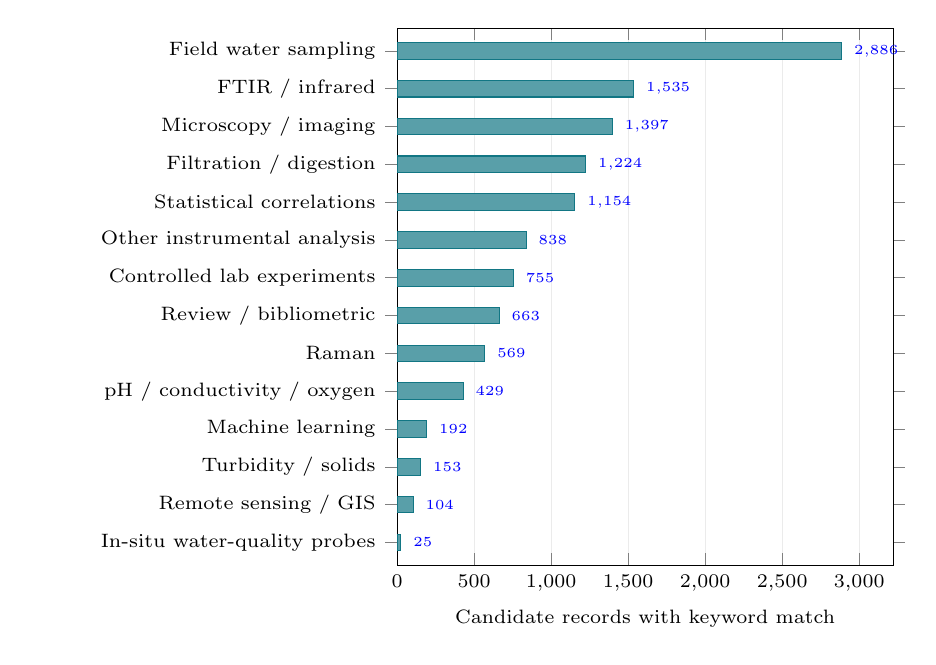
\begin{tikzpicture}
\begin{axis}[xbar,width=.65\linewidth,height=8.4cm,xmin=0,xmax=3220,ymin=-.6,ymax=13.6,
 ytick={0,...,13},
 yticklabels={{In-situ water-quality probes},{Remote sensing / GIS},{Turbidity / solids},{Machine learning},{pH / conductivity / oxygen},{Raman},{Review / bibliometric},{Controlled lab experiments},{Other instrumental analysis},{Statistical correlations},{Filtration / digestion},{Microscopy / imaging},{FTIR / infrared},{Field water sampling}},
 yticklabel style={font=\scriptsize,align=right,text width=4.3cm},tick label style={font=\scriptsize},
 xlabel={Candidate records with keyword match},xlabel style={font=\scriptsize},
 xmajorgrids=true,grid style={gray!16},bar width=6pt,
 nodes near coords,point meta=x,every node near coord/.append style={font=\tiny,anchor=west,xshift=1pt}]
\addplot+[draw=mpteal,fill=mpteal!70] coordinates {(25,0)(104,1)(153,2)(192,3)(429,4)(569,5)(663,6)(755,7)(838,8)(1154,9)(1224,10)(1397,11)(1535,12)(2886,13)};
\end{axis}\end{tikzpicture}
\caption{Original 14-category method screen ($n=6{,}654$): overlapping title/abstract matches, not confirmed experimental application or accuracy.}\label{fig:broad}
\end{figure}

\subsection{Targeted sensing and processing technologies}
A complementary search across all 10,833 candidates (title/abstract/keyword fields) found relatively few mentions of impedance/EIS (5), microfluidics (22), holography (13) and polarimetric scattering (3), compared with electrochemical sensing (55), Nile Red (138) and FTIR (1,909). Ultrasound/sonication (42) includes sample preparation; these 42 are \emph{not} 42 ultrasonic MP counters. Figure~\ref{fig:targeted} keeps this screen separate from the broader 6,654-record method classification.

\begin{figure}[H]\centering
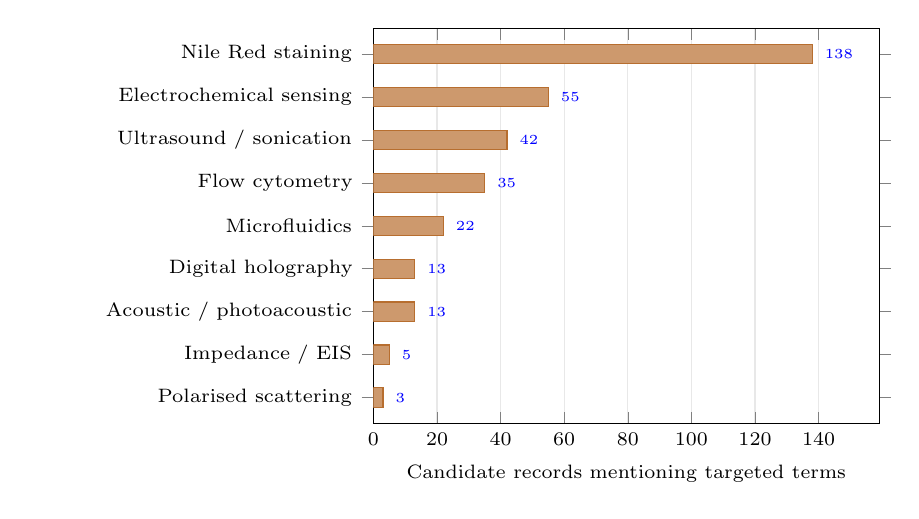
\begin{tikzpicture}
\begin{axis}[xbar,width=.66\linewidth,height=6.6cm,xmin=0,xmax=159,ytick={0,...,8},
 yticklabels={{Polarised scattering},{Impedance / EIS},{Acoustic / photoacoustic},{Digital holography},{Microfluidics},{Flow cytometry},{Ultrasound / sonication},{Electrochemical sensing},{Nile Red staining}},
 ymin=-.6,ymax=8.6,yticklabel style={font=\scriptsize,align=right,text width=4cm},tick label style={font=\scriptsize},
 xlabel={Candidate records mentioning targeted terms},xlabel style={font=\scriptsize},xmajorgrids=true,grid style={gray!18},
 nodes near coords,point meta=x,every node near coord/.append style={font=\tiny,anchor=west,xshift=1pt},bar width=7pt]
\addplot+[draw=mpgold,fill=mpgold!70] coordinates {(3,0)(5,1)(13,2)(13,3)(22,4)(35,5)(42,6)(55,7)(138,8)};
\end{axis}\end{tikzpicture}
\caption{Targeted method vocabulary in 10,833 preliminary candidates; overlap and non-detection uses are possible.}\label{fig:targeted}
\end{figure}

\subsection{Camera + AI: counting from collected or flowing water}
Lee \emph{et al.} developed skip-connection U-Net architectures for automated particle counting in microscopy images \cite{Lee2022}. Xu and Wang examined neural segmentation of urban-water MPs; these studies assess \emph{image segmentation}, not yet continuous MP particles/L accuracy on a boat \cite{UrbanCNN2024}. Choran and Ormeci investigated micro-flow imaging, including particle shape and size information in flowing samples, with bubble and matrix-related limitations \cite{Microflow2023}. A complementary flow-cytometry classification study highlights the possibility of discriminating natural particles using additional optical signatures and machine learning, at the cost of more elaborate instrumentation \cite{Wang2024}. These studies support the core concept of Track A and the image-analysis step of Track B, but they do not prove either full workflow meets the stakeholder target without further tests.

\subsection{Impedance/EIS: possible boat-mounted electrical alternative}
An electrode/flow-cell assembly applies an electrical excitation and measures a response; conventional EIS uses the complex frequency-dependent impedance $Z(f)=V(f)/I(f)$. A passing particle can perturb a confined measurement field, while dissolved salts, temperature and fouling can also dominate response. Blevins \emph{et al.} survey emerging approaches including impedance \cite{Blevins2021}. Kim \emph{et al.} used electrochemical/EIS measurements with specialised NiMoO$_4$ electrodes to detect PVC model MPs \cite{Kim2024}. Warraich \emph{et al.} studied a MXene-coated microfluidic \emph{resistance} sensor; a DC bridge is not the same as multifrequency EIS \cite{Warraich2025}. The electrical path is a \emph{research option} for Track A, but it offers no easy visual audit trail and requires rigorous salinity/particle challenge tests.

\subsection{Polarisation, fluorescence, filtration and sample concentration}
Polarised light-scattering responses have been investigated to discriminate model plastic particles from other particles, but turbidity and water matrix remain key issues \cite{Polarized2021}. Nile Red can highlight candidate MPs for camera analysis; stained organics and dye-handling logistics make it more suited to controlled shoreline post-processing than to a completely continuous, reagent-free boat sensor \cite{ErniCassola2017,Minor2023}. Portable filtration followed by digital microscopy is simpler but slow per sample and potentially vulnerable to contamination. Integrated microfluidic sample preparation has also been studied, although channel clogging and recovery remain concerns \cite{Zhang2023}. Acoustic focusing can enrich particles before a downstream detector, but enrichment alone does not identify the particles or establish the source concentration \cite{Ohori2025}.

\begin{table}[H]\centering\footnotesize
\caption{Methods selected from the candidate literature and where they fit the two workflows. \emph{Proposed fit} is an engineering judgement, not a demonstrated boat-ready product.}\label{tab:methods}
\begin{tabularx}{\linewidth}{@{}p{2.45cm}p{2.75cm}X X@{}}\toprule
Method / citation & Principle and reported setting & Track A live boat & Track B shoreline \\\midrule
Camera + U-Net \cite{Lee2022,UrbanCNN2024} & Image segmentation / particle counts from microscope images & Good AI basis; needs live flow cell, non-plastic rejection & \textbf{Very good}; image filtered/settled sample, audit individual detections \\
Micro-flow imaging \cite{Microflow2023} & Optical morphology from a flowing sample & \textbf{Good conceptual match}; optics/flow control & Useful but less essential than static microscopy \\
Nile Red + imaging \cite{ErniCassola2017,Minor2023} & Dye fluorescence enhances candidate particle contrast & Poor routine fit: reagent and waste handling & \textbf{Possible}; needs blanks, staining protocol, false-positive assessment \\
Impedance / EIS \cite{Blevins2021,Kim2024} & Electrical response to particles/interfaces & Possible experimental adjunct; high interference risk & Bench-test candidate, not needed for minimal Track B \\
Electrical microfluidics \cite{Warraich2025} & Particle-induced bridge signal in restricted channel & Potentially compact; clogging and salinity issues & Optional comparative sensor test \\
Polarised scattering \cite{Polarized2021} & Polarisation response from illuminated particles & Potential optical upgrade after camera baseline & Optional discrimination add-on \\
Filtration + portable microscopy \cite{Ermolin2024,MPWE00012} & Isolate/count imaged suspected particles from known volume & Hard to automate continuously & \textbf{Core portable reference}; membrane, blank, operator check \\
FTIR/Raman \cite{Sefiloglu2024,MPWE00012} & Spectral polymer identification & Not realistic as routine student boat payload & Not assumed available; occasional external confirmation desirable \\
Acoustic focusing \cite{Ohori2025} & Particle enrichment using acoustic force & Optional complex front-end & Possible but costly/complex compared with filtration \\
\bottomrule\end{tabularx}
\end{table}

\section{Direct comparison: strengths, weaknesses and technical risks}
\begin{table}[H]\centering\footnotesize
\caption{Trade-offs for the two deployment tracks. Advantages are conditional on successful validation.}\label{tab:proscons}
\begin{tabularx}{\linewidth}{@{}p{2.1cm}X X@{}}\toprule
Criterion & Track A: live flow-cell measurement & Track B: collected sample + shore processing \\\midrule
Main advantage & Near-continuous spatial coverage and immediate feedback; routes can be adapted & Easier to build, clean, inspect, re-count and troubleshoot; lower payload complexity \\
Main disadvantage & Optical flow stability, power draw, wet electronics, fouling and duplicate-frame counting & Delayed map; sampling is discrete; more hands-on processing \\
Typical sensors & Camera + light + flowmeter; optional polariser/EIS and water-quality probe & Portable microscope + filtration cassette + camera/AI; optional dye \\
Volume denominator & Must calibrate \emph{observed} fluid volume, not merely pump nominal throughput & Known collected volume; correct for subsampling and filter losses \\
Plastic specificity & Difficult in untreated turbid water; classifier may recognise natural fragments as plastic & Better visual access and optional stain, but still not spectroscopic polymer proof \\
Data integrity & Synchronise intake time, transit delay, frames, GPS and flow & Stable sample ID linked to GPS/time; track handling and filter IDs \\
Field practicality & More integrated engineering and maintenance risk & More achievable without lab access or expensive instrumentation \\
Map output & Updated continuously with QC; gaps where detector cannot perform & Heat map after batch processing; retain sampling points and extrapolation uncertainty \\
\bottomrule\end{tabularx}
\end{table}

\subsection{Engineering triage before buying components}
\begin{table}[H]\centering\footnotesize
\caption{Concept shortlist and decision gates; rankings are proposed project priorities, not published sensor-performance scores.}\label{tab:triage}
\begin{tabularx}{\linewidth}{@{}p{2.7cm}p{2.0cm}XX@{}}\toprule
Concept & Priority & Why it is practical & Must demonstrate first \\\midrule
B: collection + portable microscope/AI & \textbf{First prototype} & Minimal optics on boat; samples and images can be rechecked & Spike recovery, non-plastic false positives, repeatable particles/L estimate \\
A: pumped camera + AI flow cell & \textbf{Second prototype} & No return-to-shore delay; direct path to near-live map & Calibrated observed volume, focus, frame de-duplication, matrix robustness \\
A: EIS / microfluidic electrical sensor & Feasibility side-test & Small possible footprint and fast electronics & MP discrimination across salinity, sediment, size; event count vs bulk response \\
RGB turbidity / conductivity proxy & Auxiliary only & Cheap and easy to mount on boat & Out-of-sample correlation with verified MP count; uncertainty and confounder tests \\
\bottomrule\end{tabularx}
\end{table}

\section{Validation without routine laboratory equipment}
\subsection{The scientific boundary}
The stakeholder still requires reliable estimates demonstrably related to actual MPs. A camera trained on shape alone counts \emph{MP-like particles}, and a conductivity sensor measures ionic electrical properties. Neither can prove polymer identity in an unknown environmental sample on its own. Therefore the team should separate three validation goals: \emph{(i)} count known test particles, \emph{(ii)} reject non-plastic interferents, and \emph{(iii)} establish polymer-specific credibility using occasional external standards/confirmation if at all available. If the third goal is not met, label the map ``estimated/suspected MP-like particle concentration'' rather than certified MP concentration \cite{Blevins2021,ErniCassola2017,Ermolin2024}.

\subsection{Portable experiments the team can perform}
\begin{table}[H]\centering\footnotesize
\caption{Low-infrastructure validation plan suitable for bench, shoreline and boat trials; targets must be set experimentally.}\label{tab:verification}
\begin{tabularx}{\linewidth}{@{}p{2.7cm}X X@{}}\toprule
Test & How to conduct it without specialist chemistry equipment & Required record / failure indicator \\\midrule
Blanks and contamination & Run filtered-water and empty-cassette controls; cover samples, use clean handling, record blank detections & Blank particle count and field contamination events \\
Known-particle dilution & Prepare known-volume suspensions of characterised PE/PP/PS beads/fragments at several levels; repeat & Measured-vs-expected counts, bias, recovery, detection limits \\
Non-plastic challenge & Independently add silt, algae and bubbles in MP-free water and mixed suspensions & False-positive/negative rates and how accuracy changes with water matrix \\
Size, speed and volume & Vary particle sizes, pump speed, optical focus and sample volumes & Detectable size range, flow cell volume, repeat counting rate \\
Independent image review & Blindly re-label a subset of raw images by human operators; repeat on different days & Precision/recall, disagreements, drift and repeatability \\
Shoreline method agreement & Split paired field samples between Track A and Track B; compare blind outputs & Agreement, MAE/RMSE and location-specific errors \\
External polymer spot-check (optional) & Send only a small stratified sample of recovered particles to a university/collaborator when feasible & Polymer-confirmation rate; record unavailable if not done \\
\bottomrule\end{tabularx}
\end{table}

For Track A, the denominator must correspond to \emph{fluid actually observed} by the image sensor: $\widehat{C}_{A}=N_{\mathrm{unique,classified}}/V_{\mathrm{imaged}}$. For Track B, $\widehat{C}_{B}=(N_{\mathrm{counted}}-N_{\mathrm{blank}})/(V_{\mathrm{collected}}\,r)$ only when a defensible recovery fraction $r$ is measured and the entire analysed fraction is accounted for. Until polymer specificity is validated, both concentrations are \emph{suspected MP-like counts per litre}. Blank correction and recovery uncertainty must not be silently assumed.

\subsection{Heat-map generation and communication}
The software takes $(\mathrm{lat},\mathrm{lon},t,V,N,\mathrm{QC})$ from either track, computes a concentration estimate and displays \emph{actual measured locations} before optional spatial interpolation. Each map needs a legend with units, a declared size cutoff, an explicit timestamp/survey period, sample density and unsupported areas. Interpolate only within supported coverage. Compare prediction values against a subset of \emph{withheld} sample stations; do not validate the interpolation using exactly the same stations on which it was fitted. Real-time maps and shore-processed maps should use the same schema so their performance can be compared directly.

\section{Recommended next steps and decision milestones}
\begin{enumerate}
\item \textbf{Specify the measurand.} Set target size fraction and concentration units (particles/L, not area-normalised count unless explicitly justified). Choose whether the first prototype is for suspected MPs rather than polymer-certified MPs.
\item \textbf{Pilot Track B first.} Build clean collection cassettes, sample IDs, measured-volume collection, portable image capture, simple AI/threshold counting and GPS-linked CSV/map output.
\item \textbf{In parallel, prototype Track A optics.} Pump through a transparent chamber; evaluate video quality, one-particle/one-count tracking, tubing-delay correction and cleaning effort on the same known-particle dilutions.
\item \textbf{Use EIS only as a gated side experiment.} Compare known MPs against salt, sediment and non-plastics; stop early if signals are dominated by water conductivity or unstable electrode effects.
\item \textbf{Field trial both tracks.} Survey a modest route with replicated paired samples, contamination blanks and withheld locations; quantify device agreement and heat-map error.
\item \textbf{Go/no-go decision.} Prefer Track A only if its extra automation produces trustworthy counts and repeatable operation; otherwise Track B can still satisfy the spatial-map objective through rapid shoreline post-processing. Seek limited independent polymer confirmation to support any claim of true MP concentration.
\end{enumerate}

\section{Limitations of this working literature review}
The evidence base is a \emph{preliminary title/abstract candidate pool}. Automated categories overlap; a matched keyword does not establish experimental deployment, evidence quality or causal relationships. Selected cited papers illustrate operating principles and performance issues but are not a quantitative meta-analysis of all 10,833 papers. Detailed performance figures and protocols must be checked against full texts before a final thesis. The proposed tracks, tests and prioritisation are engineering recommendations motivated by the stakeholder brief and the reviewed candidate literature.

\printbibliography[title={References}]
\end{document}